\documentclass[a4paper]{instrumentacao}

\usepackage{etoolbox}
\usepackage{float}

\newtoggle{attachments}
\toggletrue{attachments}

\extrafloats{100}

\graphicspath{
	{../Resources/Images/}
	{../Resources/Mathematica/images/}
	{../Resources/MATLAB/images/}
}

\title{Simulação e Experimentos com Células de Cargas}
\author{Rogiel Sulzbach \and Rodrigo de Castro Silveira}
\startdate{02/05/2016}
\finishdate{30/05/2016}
\emails{
	\emailaddress{R.J.S.}{rogiel@rogiel.com},
	\emailaddress{R.C.S.}{csilveira.rodrigo@gmail.com}
}

\resume{}
\abstract{} 
\keywords{}
\institute{}

\headertext{Extensometria}

\begin{document}
\maketitle

\chapter{Introdução}

Nesta atividade de relatório foram feitas várias atividades de laboratório utilizando sensores do tipo extesômetro. Um extensômetro é um sensor resistivo cuja resistência elétrica varia com a deformação mecânica do sensor. A Figura \ref{fig:intro-extensometro} apresenta um extensômetro do tipo grade:

\begin{figure}[H]
\center
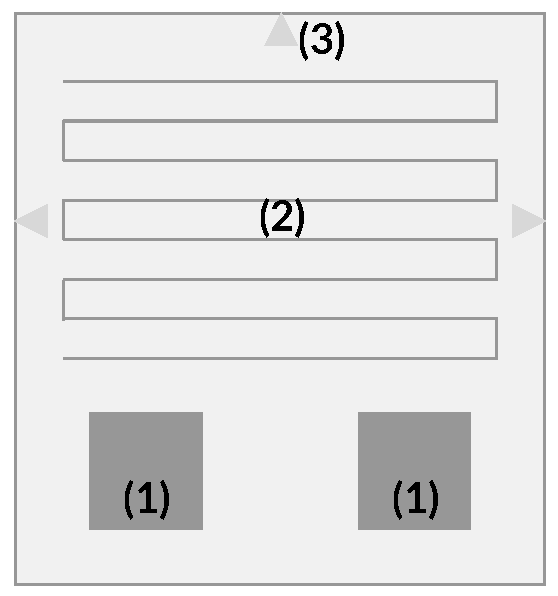
\includegraphics[width=0.5\textwidth]{ExtensometroGrade.pdf}
\caption{Desenho simplificado de um extensômetro do tipo grade}
\label{fig:intro-extensometro}
\end{figure}

\noindent onde (1) representa os \textit{pads} de conexão elétrica do sensor, (2) é a grade do sensor e (3) são os indicadores de alinhamento do sensor. Este tipo de extensômetro é dito como uniaxial pois deformações fora do seu eixo principal são insignificantes perto da variação de resistência elétrica devido à deformações ao longo do seu eixo principal.

Conforme apresentado na Figura \ref{fig:intro-extensometro} a grade do sensor (2) é composta por um material condutor com uma resistência elétrica característica. Uma vez que o sensor esteja cimentado (colado) sobre uma superfície deformações na superfície se propagam como deformação do sensor que deformam a grade. Deformações na grade causam pequenas alterações (na ordem de $10^{-6} \Omega$) na resistência elétrica do sensor. Com um circuito elétrico de condicionamento adequado, estas pequenas variações de resistência elétrica do sensor podem ser medidas e quantificadas em valores de deformação mecânica.

Os indicadores de alinhamento do sensor (3) conforme apresentados na figura \ref{fig:intro-extensometro}, indicam o ponto de maior sensibilidade do sensor, isto é, onde há a maior variação de resistência elétrica para uma mesma deformação.

O extensômetro pode ser modelado matematicamente de forma simplificada pela Equação \ref{eq:intro-extensometro}:

\begin{equation}
	\frac{\Delta R}{R_0} = k \frac{\Delta l}{l_0} = k\epsilon
	\label {eq:intro-extensometro}
\end{equation}

\noindent onde $\Delta R/R_0$ é a variação relativa de resistência elétrica do sensor referente ao seu valor inicial de repouso (ou nominal) $R_0$, $\Delta l/l_0$ é a deformação mecânica relativa do sensor referente ao seu valor inicial de repouso (ou nominal) $l_0$ também definida como $\epsilon$ e $k$ é uma constante que define a relação entre variação de resistência elétrica e deformação do sensor, conhecido como fator \textit{gage}.

Dessa forma, é possível relacionar a deformação mecânica da grade do sensor com a variação de resistência elétrica do sensor. Como a variação de resistência elétrica é muito baixa (ordem de $10^{-6}$) para que seja possível medir esta variação é necessário que se utilize um circuito de condicionamento de qualidade. Uma topologia muito comum é a utilização da ponte de Wheatstone, que dá origem a 3 montagens comuns com extensômetros: 1/4 de ponte, meia ponte e a ponte completa.

Este relatório versará sobre experimentos utilizando células de carga, onde será levantada a função de transferência experimental para uma célula de carga comercial da HBM e outra célula de carga não-comercial feita com uma simples barra de alumínio e extensômetros cimentados sobre a barra que será validado utilizando um modelo computacional simulado. Adicionalmente foi levantada a função de transferência experimental de um torquímetro disponível no laboratório.

Como a variação de resistência elétrica em extensômetros é observada em um valor tão baixo (ordem de $\mu\Omega$), o circuito de condicionamento é fundamental e portanto uma breve análise em circuitos de condicionamento será feita.

\chapter{Metodologia Experimental}
Nestes experimentos de laboratório foi utilizado o software Wolfram Mathematica 10.4.0 da Wolfram Research, Inc. para realizar todos os cálculos no computador utilizando precisão do tipo MachinePrecision\cite{mathematica-numerial-precision} onde a precisão dos números de ponto flutuante respeitam os critérios impostos pelo processador (64 bits, precisão dupla) que implementam o padrão IEEE de ponto flutuante, possuem um "Épsilon de Máquina", o menor valor que somado a 1 retorna um valor diferente de 1, isto é, não causa arredondamento \cite{wikipedia-epsilon}, de $2^{-52}$, ou seja, na ordem de $10^{-16}$ e podem, portanto, serem desprezados perante a resolução de todos os outros instrumentos utilizados no experimento. Adicionalmente, quando possível, os cálculos foram realizados de forma simbólica com substituição numérica no final. Os scripts utilizados para cálculo estão anexados ao fim do documento, na Página \pageref{ch:attachments}.

Para a realização de simulações mecânicas do modelo computacional 3D foi utilizado o software SOLIDWORKS 2016 SP2 desenvolvido pela Dassault Systèmes SolidWorks Corp.

\section{Célula de carga comercial}

Neste experimento foi levantada a função de transferência experimental para uma viga engastada utilizando uma célula de carga comercial \todo{marca e outros detalhes da célula}.

Na Figura \ref{fig:celula-comercial-circuito} está apresentado o esquemático elétrico de uma ponte de Wheatstone:

\begin{figure}[H]
\center
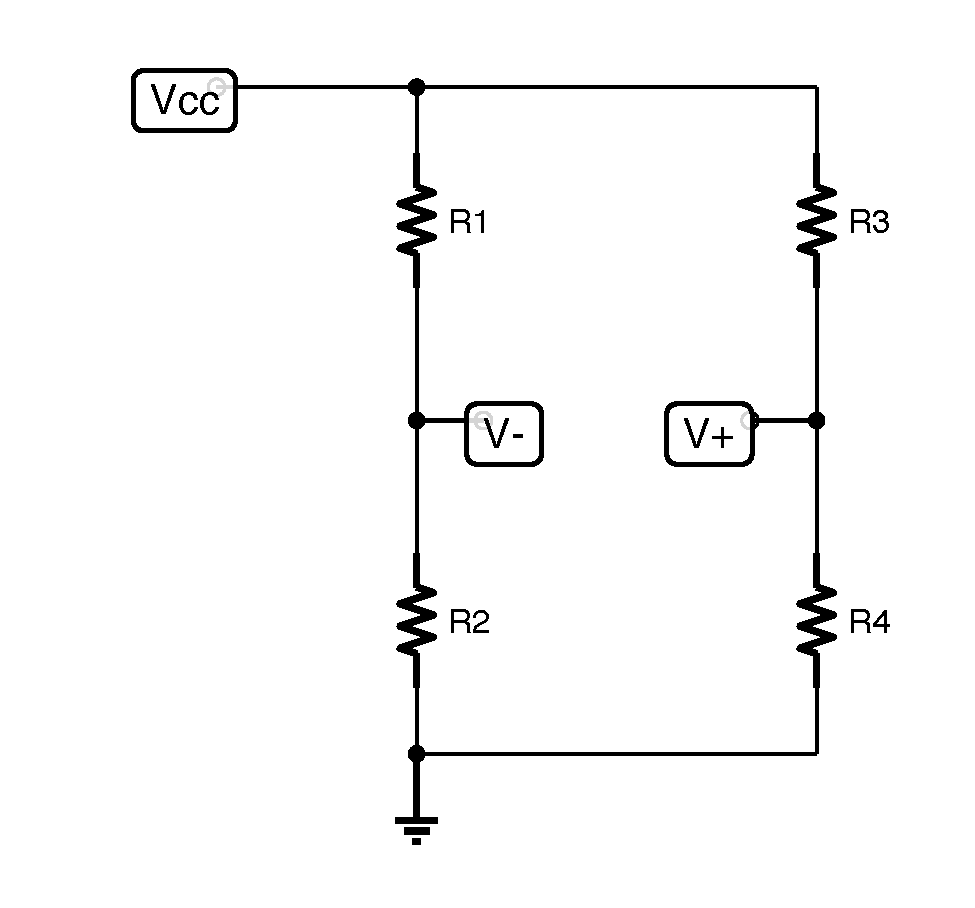
\includegraphics[width=\textwidth]{Wheatstone.pdf}
\caption{Esquemático elétrico de uma ponte de Wheatstone genérica.}
\label{fig:celula-comercial-circuito}
\end{figure}

\noindent onde os resistores $R_1$, $R_2$, $R_3$ e $R_4$ são valores de resistência elétrica que determinam o comportamento de ponte, $V_-$ e $V_+$ são os nós de saída da ponte medidos em tensão elétrica e $V_{cc}$ é a tensão elétrica de alimentação da ponte.

A função de transferência da ponte de Wheatstone proposta é dada conforme Equação \ref{eq:wheatstone-tf}:

\begin{equation}
	V_o = V_+ - V_- = \left(\dfrac{R_4}{R_4 + R_3} - \dfrac{R_2}{R_1 + R_2}\right)V_{cc}
	\label{eq:wheatstone-tf}
\end{equation}

Considerando que as condições das Equações \ref{eq:celula-comercial-cond1} e \ref{eq:celula-comercial-cond2} são válidas, então a ponte é dita estar "em equilíbrio", isto é, a saída de tensão elétrica entre $V_-$ e $V_+$ é de $0V$.

\begin{eqnarray}
	R_1 = R_3 \label{eq:celula-comercial-cond1} \\
	R_2 = R_4 \label{eq:celula-comercial-cond2}
\end{eqnarray} 

Qualquer pequena variação de resistência elétrica em qualquer um dos resistores da Figura \ref{fig:celula-comercial-circuito} que violem as condições da Equação \ref{eq:celula-comercial-cond1} e \ref{eq:celula-comercial-cond2} incorre no desequilíbrio da ponte, que pode ser medido utilizando a saída em tensão elétrica.

Com isto, a ponte pode ser utilizada como circuito de condicionamento para um sistema de medição de deformação mecânica de um corpo. Na Figura \ref{fig:celula-comercial-esquema-fisico} está apresentado um esquemático físico da célula de carga comercial utilizada:

\begin{figure}[H]
\center
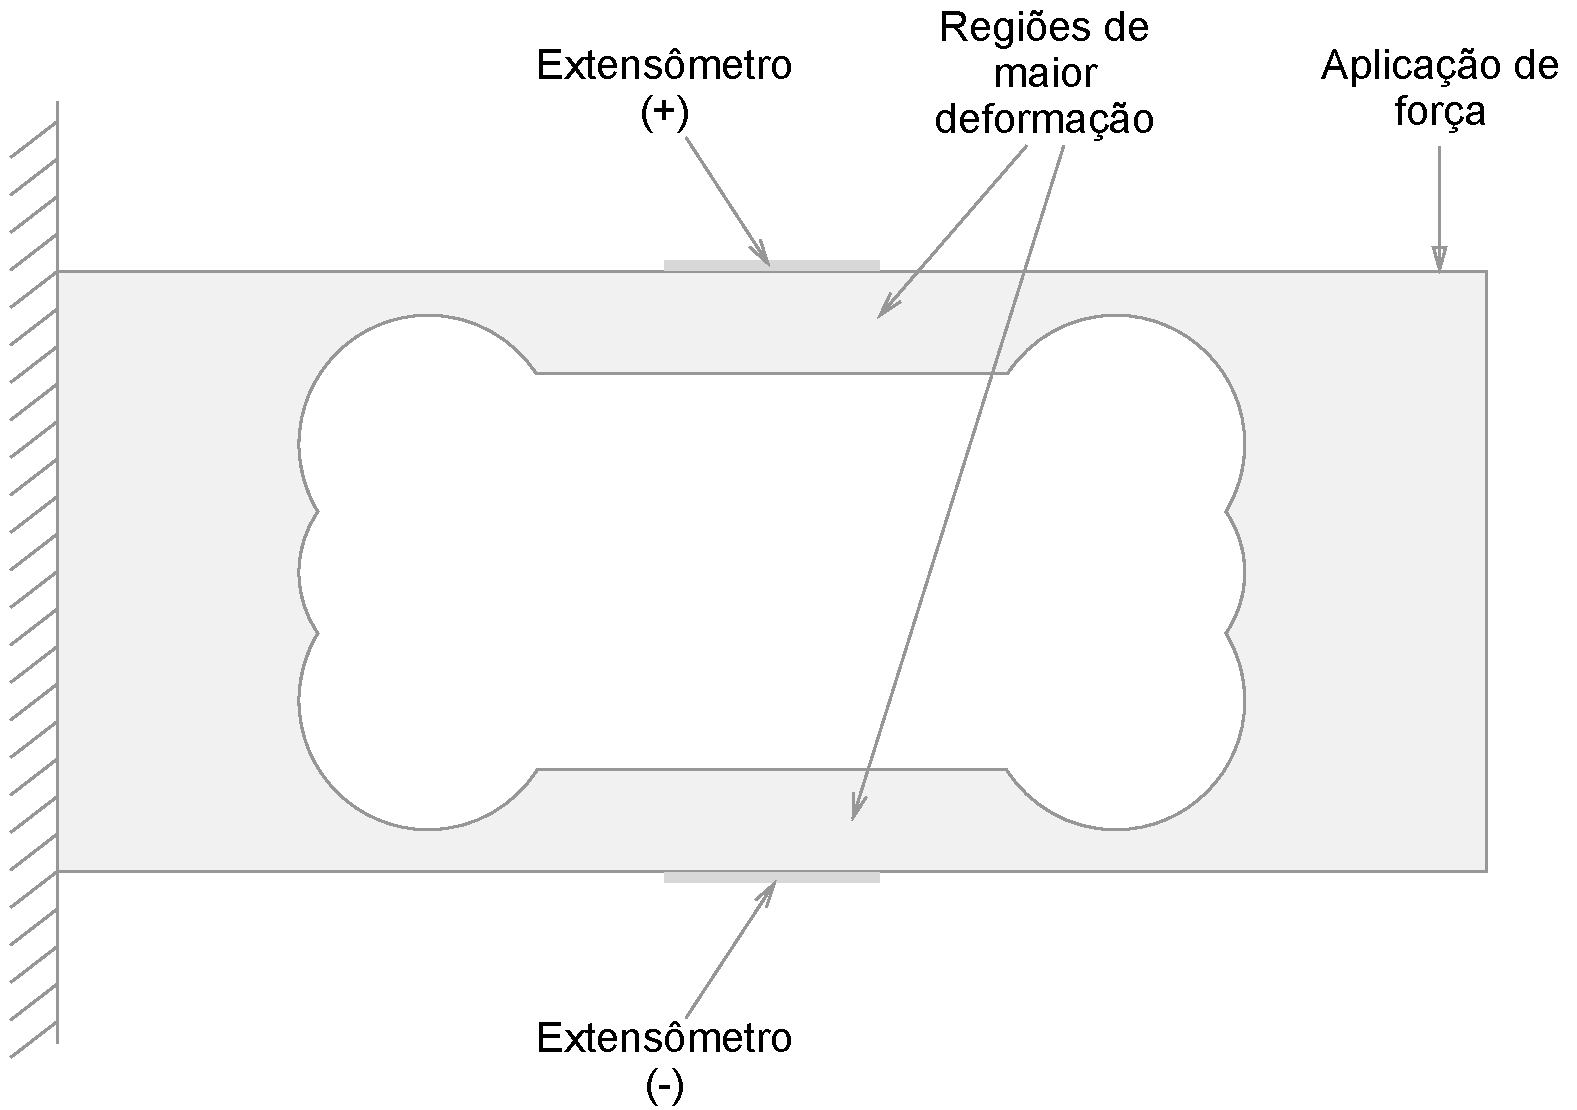
\includegraphics[width=\textwidth]{CelulaComercial.pdf}
\caption{Esquemático da construção mecânica da célula de carga comercial utilizada no experimento.}
\label{fig:celula-comercial-esquema-fisico}
\end{figure}

\noindent onde o extensômetro $(+)$ indica uma deformação positiva (alongamento) e o extensômetro $(-)$ indica uma deformação negativa (compressão).

Portanto, é possível utilizar esta construção como forma de medir deformações que a viga proposta esteja submetida. É comum utilizar 3 formas distintas de medição utilizando extesômetros e a ponte de Wheatstone.

\todo{continuar}

De acordo com o fabricante a sensibilidade da célula é de $2 mV/V$ e possui $350 \Omega$ de resistência elétrica nominal e com carga máxima de $5 kg$.  O fabricante da célula é "FLEXAR Celdas de Carga", um fabricante argentino de células de carga, modelo "REACCION BCD-5". O site do fabricante não possuía listagem com especificações técnicas deste modelo e portanto não há informações mais detalhadas sobre esta célula, como incertezas da resistência nominal, incerteza da sensibilidade e outros detalhes.

Todas medidas de tensão elétrica da célula foram feitas utilizando o LabVIEW versão 7.1 disponibilizada pelo laboratório com auxílio dos dispositivos de DAQ da National Instruments modelo USB-6009. Conforme o fabricante \cite{daq-specifications} a entrada analógica deste dispositivo possui 14 bits, taxa de amostragem de 48 kS/s e resolução de tensão elétrica de 1.53mV. O sinal de saída foi amostrado à uma taxa de 1000 Hz com 500 amostras e a média destes valores era tomado como uma única medida experimental. Este processo visa minimizar o impacto do ruído aditivo gaussiano branco (AWGN) gerado pelo circuito de condicionamento na medida realizada.

O circuito de condicionamento consistia em um amplificador de instrumentação (AI) INA126AP fabricado pela Texas Instruments com \textit{bias} de corrente de entrada máxima de 25 nA \cite{datasheet-ina126} configurado com ganho de \todo{quanto?}. O circuito de condicionamento foi alimentado utilizando um regulador de tensão elétrica positivo LM7805 de $5V \pm 0,2V$ \cite{datasheet-lm7805} fabricado pela Fairchild Semiconductors e com um regulador de tensão elétrica negativo LM7905 de $-5V \pm 0,2V$ \cite{datasheet-lm7905} fabricado pela Texas Instruments. A célula de carga foi alimentada utilizando a referência de tensão elétrica REF02 de $5V \pm 0,01V$ \cite{datasheet-ref02} fabricado pela Texas Instruments.

A Figura \ref{fig:celula-comercial-metodologia-condicionamento} apresenta o esquemático elétrico do circuito de condicionamento da célula de carga.

\begin{figure}[H]
\center
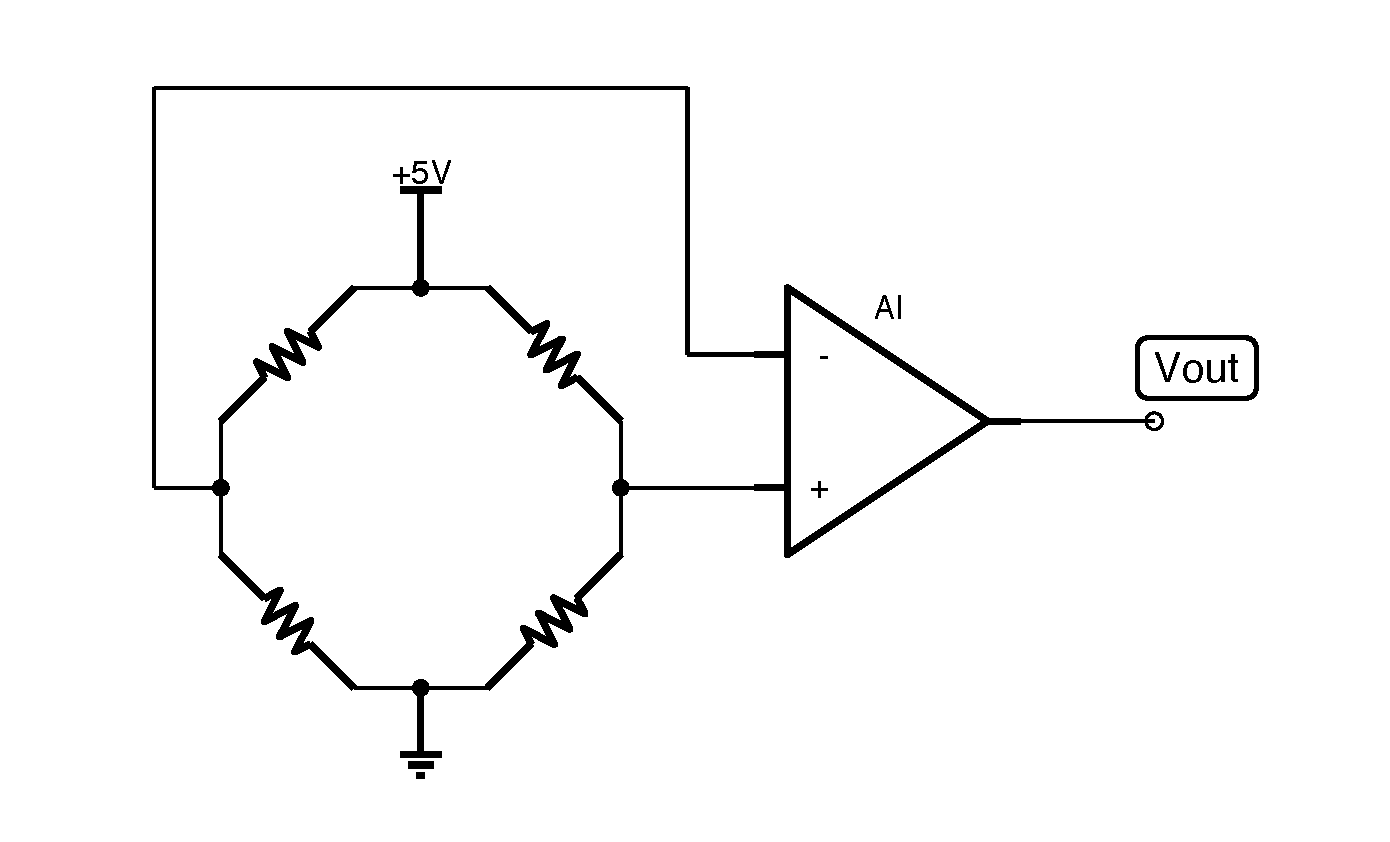
\includegraphics[width=\textwidth]{Comercial-Circuito.pdf}
\caption{Esquemático elétrico do circuito de condicionamento da célula de carga comercial}
\label{fig:celula-comercial-metodologia-condicionamento}
\end{figure}

\noindent onde a alimentação de $+5V$ representa a referência de tensão elétrica REF02, os resistores representam de forma simbólica a ponte de Wheatstone interna da célula de carga (o fabricante não informa de forma exata a topologia de construção da ponte nem valores de resistores que colaboram no balanço da ponte), o amplificador AI é um amplificador de instrumentação com ganho de \todo{quanto?} e $V_{out}$ é a tensão elétrica de saída da ponte, filtrado, amostrado pelo DAQ e medido no LabVIEW.

O circuito de amostragem consistia em um filtro passa-baixas de Butterworth de ordem 4 com frequência de corte de 100Hz utilizando a topologia de filtros analógicos ativos de Sallen-Key. Como amplificador operacional para a implementação do filtro, utilizou-se o amplificador operacional encapsulado TL084 da Texas Instruments com distorção harmônica total típica de $0,003\%$ \cite{datasheet-tl084}.

A Figura \ref{fig:celula-comercial-cadeia-transducao} apresenta a cadeia de transdução completa utilizada no experimento.

\begin{figure}[H]
\center
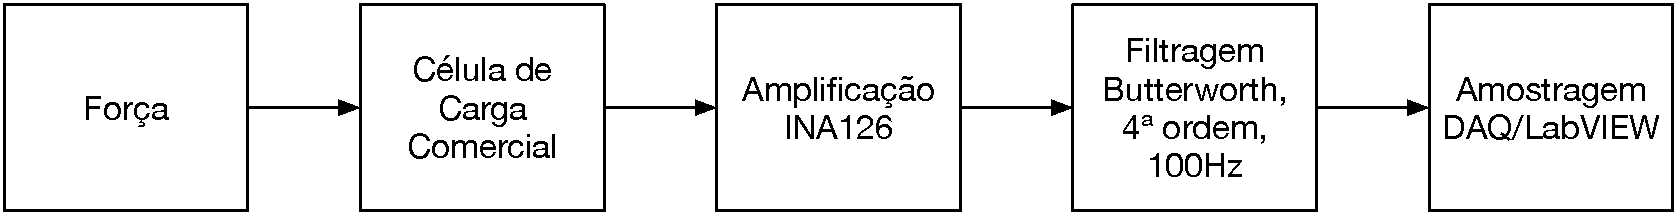
\includegraphics[width=\textwidth]{Comercial-Cadeia-Transducao.pdf}
\caption{Cadeia de transdução completa do experimento com a célula de carga comercial}
\label{fig:celula-comercial-cadeia-transducao}
\end{figure}

\todo{cadeia de medida}

\section{Célula de carga não-comercial}

A célula de carga não comercial utilizada possuía a configuração dada na Figura \ref{fig:celula-nao-comercial-desenho}:

\begin{figure}[H]
\center
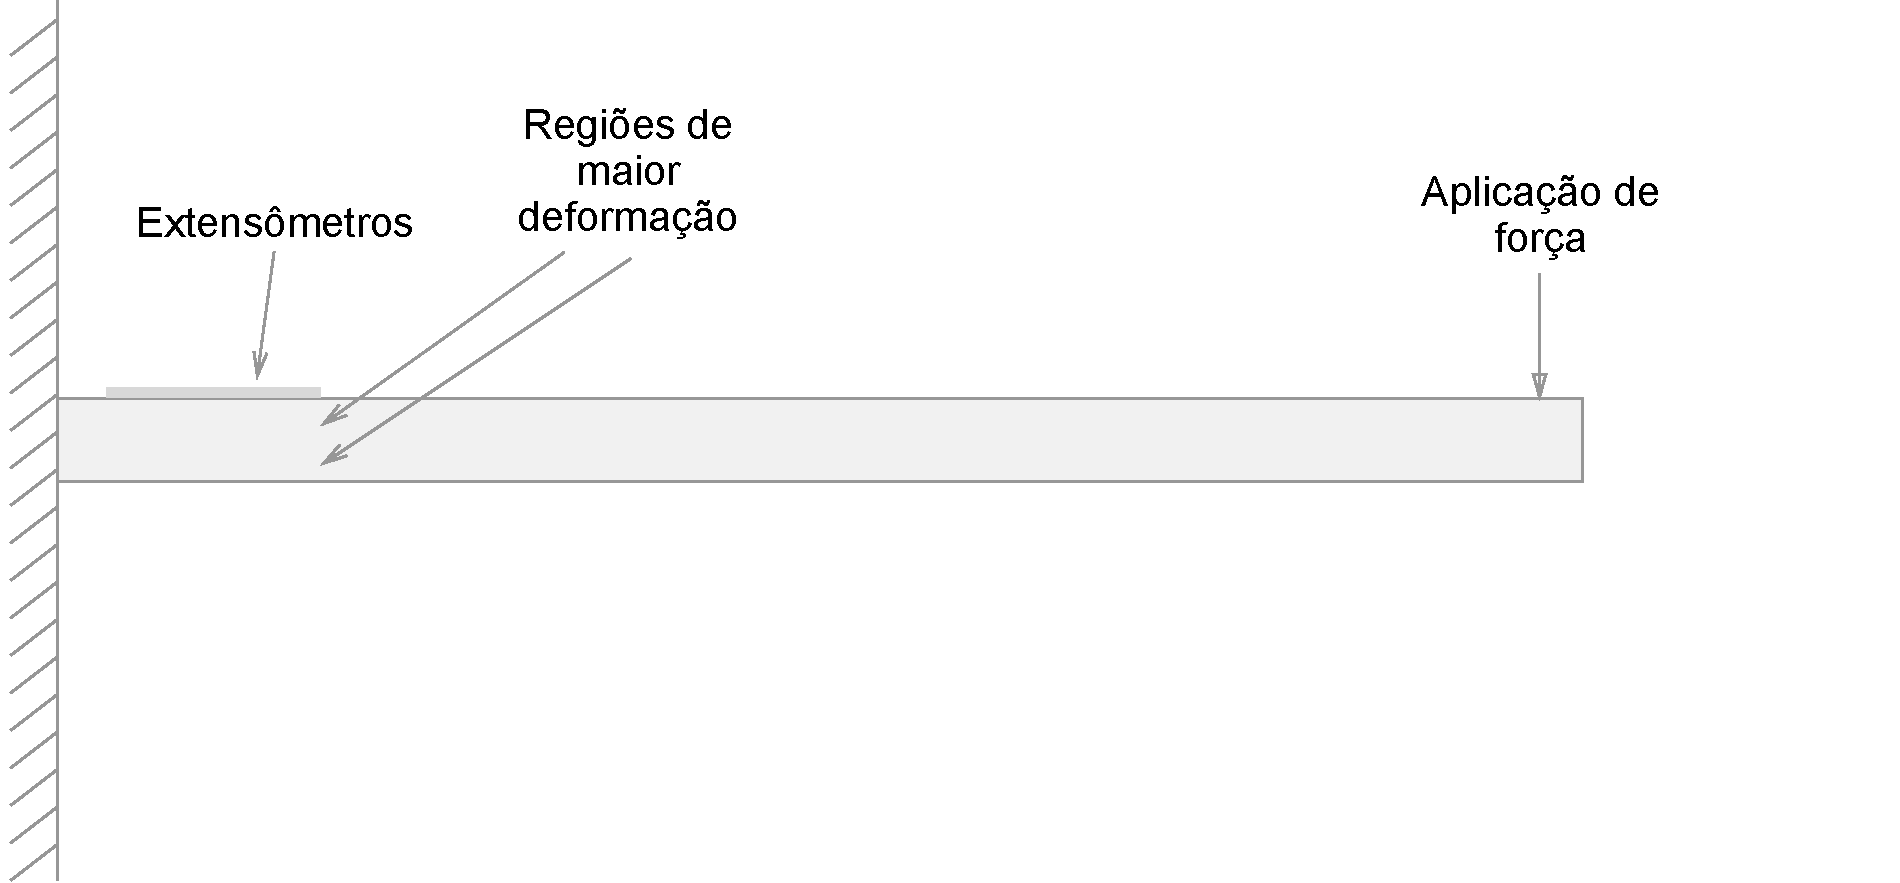
\includegraphics[width=\textwidth]{CelulaNaoComercial.pdf}
\caption{Esquemático da construção mecânica da célula de carga não-comercial utilizada no experimento.}
\label{fig:celula-nao-comercial-desenho}
\end{figure}

\noindent onde o extensômetro $(+)$ indica uma deformação positiva (alongamento) e o extensômetro $(-)$ indica uma deformação negativa (compressão). É importante observar que a célula possuía um extensômetro na parte superior (próximo à base de suporte) e outro extensômetro na mesma posição, mas na face inferior da barra. Em termos prático, isto significa que para uma mesma deformação, o variação de resistência elétrica em ambos os extensometros é idêntica em módulo, mas com diferente sinal. Este comportamento é importante pois espera-se que a saída da ponte de Wheatstone fique constante com o aquecimento da barra, fato que não aconteceria caso fosse utilizada a mesma face da ponte para a colagem dos extensômetros.

Ao contrário da célula comercial, esta nao possui a ponte pré-calibrada e, portanto, se fez necessário que a ponte fosse calibrada e ajustada para obter o resultado desejado. De acordo com a especificação dos extensômetros (modelos e fabricantes não estavam explícitos sobre a construção, logo, não foi possível comparar com os valores fornecidos pelo fabricante). Havia, contudo, uma marcação indicando o valor de resistência nominal do extensômetro.

Considerando que a resistência elétrica nominal da célula de carga quando em repouso seja de $350 \Omega$ com incerteza desconhecida, é possível calcular os resistores para os demais braços da ponte de Wheatstone. A Figura \ref{fig:celula-nao-comercial-ponte}

\begin{figure}[H]
\center
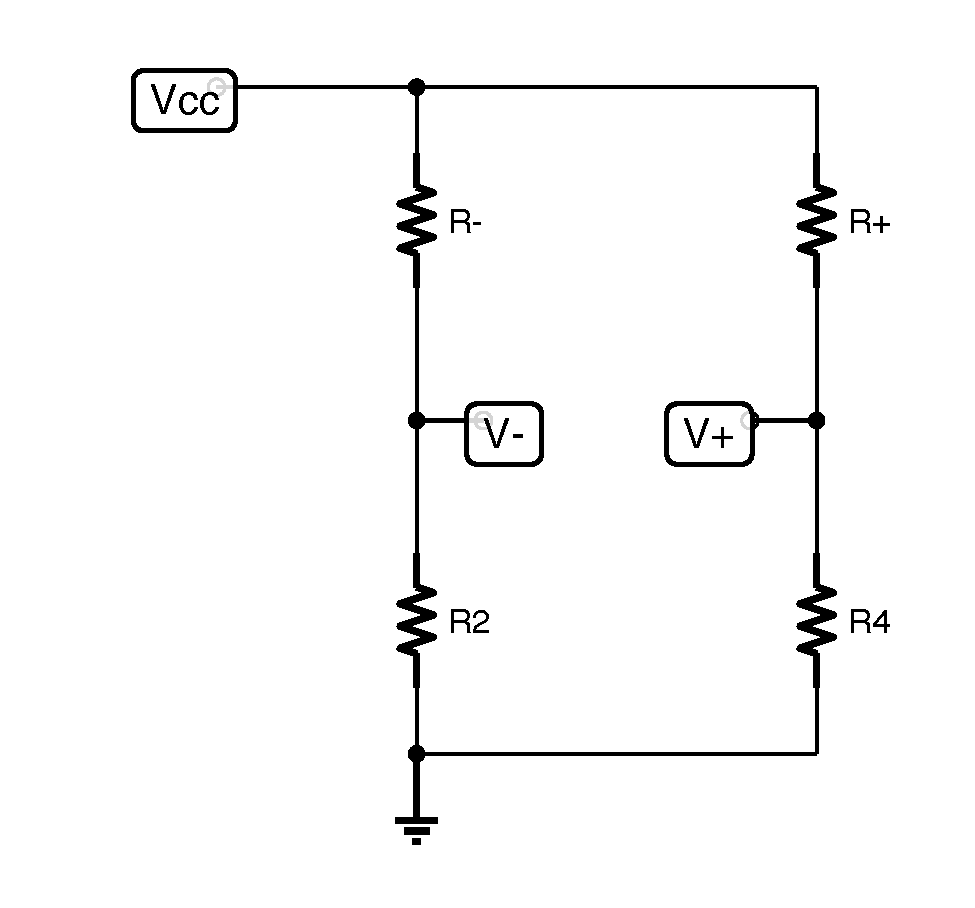
\includegraphics[width=\textwidth]{WheatstoneNaoComercial.pdf}
\caption{Esquemático elétrico da ponte de Wheatstone para a célula de carga não-comercial. O modelo escolhido foi utilizar uma meia-ponte, com variação positiva e outra negativa.}
\label{fig:celula-nao-comercial-ponte}
\end{figure}

\noindent onde os resistores $R_2$ e $R_4$ são resistores cujo valor deve ser o mais próximo possível do valor nominal dos extensômetros da ponte e $R+$ e $R-$ são os extensômetros com variação, respectivamente, positiva e negativa, de resistência elétrica em função da deformação da barra.

\subsection{Modelo computacional}
A fim de realizar uma validação computacional dos resultados, foi desenvolvido um modelo computacional para a célula de carga não-comercial no software SOLIDWORKS 2016 x64 e realizada utilizando o método FFEPlus com a opção de \textit{large displacement} desativada.

Na simulação de análise estática da célula, foi aplicada uma força de ??? N \todo{quanto?} sobre o furo presente na barra. A Figura \ref{fig:celula-nao-comercial-solid-modelo} apresenta o modelo 3D desenvolvido no software:

\begin{figure}[H]
\center
%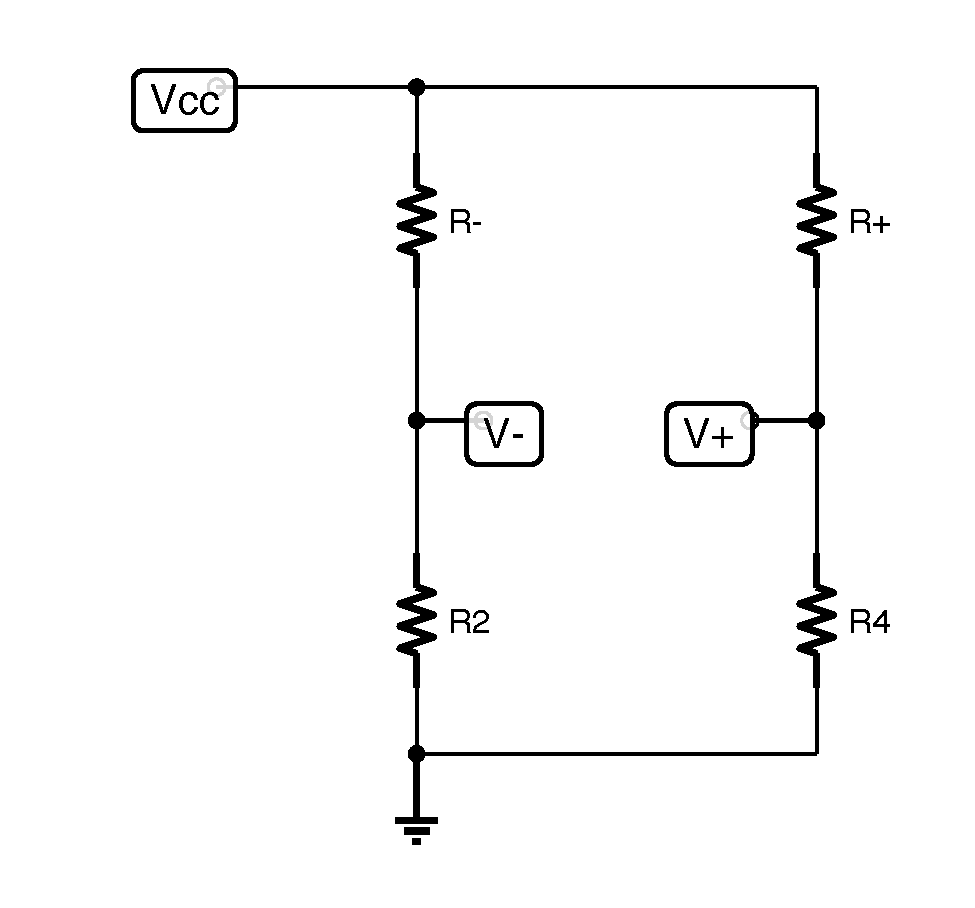
\includegraphics[width=\textwidth]{WheatstoneNaoComercial.pdf}
...
\caption{Modelo 3D utilizado para a simulação da célula de carga não-comercial no SOLIDWORKS.}
\label{fig:celula-nao-comercial-solid-modelo}
\end{figure}
\todo{figura solid}

\noindent onde a superfície de aplicação da força é o orifício utilizado para exercer as forças durante a execução do experimento no laboratório.

Nesta simulação foi possível estimar a deformação da barra para os valores de 2N, 4N, 6N, 8N e 10N que correspondem, aproximadamente aos pesos das massas de 200g, 400g, 600g, 800g e 1kg (considerando que a aceleração local da gravidade $g$ é dada, aproximadamente, por $10 m/s^2$.

A fim de determinar a frequência fundamental da vibração do sistema, foi realizada uma simulação dinâmica de frequência do sistema. Nesta simulação a frequência fundamental de vibração do sistema foi extraída e validada com o experimento em que uma batida é feita na barra e pela vibração medida pelo extensômetro é possível estimar a frequência fundamental de vibração do sistema.

\section{Torquímetro}
Neste experimento foi utilizado um torquímetro cujo ponto de maior torque (no eixo do torquímetro) haviam 4 extensômetros cimentados nos 4 lados do metal do cabo, portanto uma ponte completa. Com este sistema, é possível medir o toque exercido pelo operador no instrumento.

O torquímetro já estava construído e possuía 4 fios: 2 de alimentação (terra e alimentação positiva) e outros 2 fios para a saída: positivo e negativo. Para extrair a função de transferência do torquímetro foi aplicado torque utilizando o medidor físico gravado sobre o instrumento nos valores \todo{quais valores de torque?}

\chapter{Resultados e Discussões}

\section{Célula de carga comercial}
A Tabela \ref{tab:celula-comercial-resultado-funcao-transferencia} apresenta as medidas experimentais para a célula de carga comercial.


\begin{table}[H]
\centering
\caption{Tabela com os valores de medidos experimentalmente para ajuste da função de transferência experimental da célula de carga comercial.}
\begin{tabular}{|l|l|l|}

\hline
\textbf{Massa (kg)} & \textbf{Medida \#1 (V)} & \textbf{Medida \#2 (V)} \\ \hline
0.0 & 1.899 & 1.896 \\ \hline
0.2 & 1.887 & 1.885 \\ \hline
0.4 & 1.875 & 1.867 \\ \hline
0.6 & 1.863 & 1.858 \\ \hline
0.8 & 1.852 & 1.846 \\ \hline
1.0 & 1.841 & 1.834 \\ \hline
1.2 & 1.823 & 1.827 \\ \hline
1.4 & 1.818 & 1.811 \\ \hline
1.6 & 1.806 & 1.799 \\ \hline
1.8 & 1.795 & 1.788 \\ \hline
2.0 & 1.784 & 1.781 \\ \hline
2.2 & 1.766 & 1.769 \\ \hline
2.4 & 1.760 & 1.757 \\ \hline
2.6 & 1.748 & 1.743 \\ \hline
2.8 & 1.737 & 1.734 \\ \hline
3.0 & 1.724 & 1.718 \\ \hline
3.2 & 1.708 & 1.712 \\ \hline
3.4 & 1.702 & 1.695 \\ \hline
3.6 & 1.691 & 1.684 \\ \hline
3.8 & 1.679 & 1.671 \\ \hline
4.0 & 1.668 & 1.665 \\ \hline
4.2 & 1.652 & 1.654 \\ \hline
4.4 & 1.644 & 1.642 \\ \hline
4.6 & 1.631 & 1.631 \\ \hline
4.8 & 1.621 & 1.619 \\ \hline
5.0 & 1.609 & 1.608 \\ \hline

\end{tabular}
\label{tab:celula-comercial-resultado-funcao-transferencia}
\end{table}

A função que melhor ajusta os dados da Tabela \ref{tab:celula-comercial-resultado-funcao-transferencia} é dada na Equação \ref{eq:celula-comercial-resultado-funcao-transferencia}

\begin{equation}
	m(V) = 32.9198 - 17,3681 V
	\label{eq:celula-comercial-resultado-funcao-transferencia}
\end{equation}

\noindent onde $m(V)$ é a massa em $kg$ a qual a viga está submetida e $V$ é a tensão elétrica em $V$ medida na saída de ponte de Wheatstone com o sensor.

A função foi ajustada com $R^2$ dado pela Equação \ref{eq:celula-comercial-resultado-funcao-transferencia-r2}

\begin{equation}
	R^2 = 0.998975
	\label{eq:celula-comercial-resultado-funcao-transferencia-r2}
\end{equation}

\todo{erro de linearidade}

A Figura \ref{fig:celula-comercial-resultado-funcao-transferencia} apresenta um gráfico com a função de transferência da Equação \ref{eq:celula-comercial-resultado-funcao-transferencia} e os dados da Tabela \ref{tab:celula-comercial-resultado-funcao-transferencia}.

\begin{figure}[H]
\center
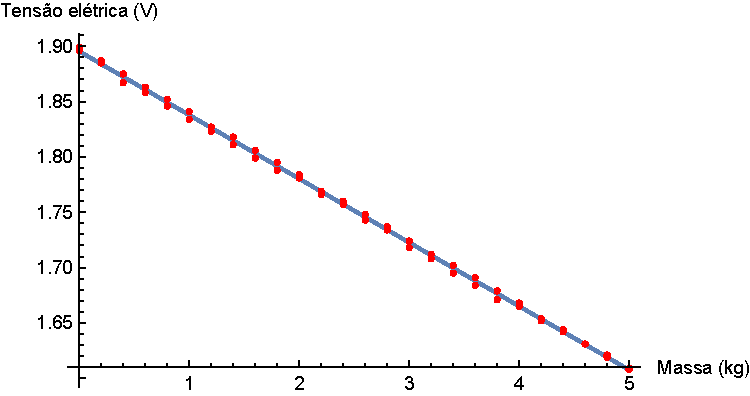
\includegraphics[width=\textwidth]{Comercial-Plot.pdf}
\caption{Função de transferência experimental: função de melhor ajuste e medidas experimentais}
\label{fig:celula-comercial-resultado-funcao-transferencia}
\end{figure}

\noindent onde a linha contínua representa a função ajustada e os pontos representam cada medida individual realizada.

Com a função de transferência é possível aplicá-la nos dados adquiridos em laboratórios e obter a resposta da célula para a adição ou remoção de carga.

A Figura \ref{fig:celula-comercial-resultado-0-1kg} apresenta a resposta da célula quando adicionado um peso suspenso  de $1 kg$ na barra. Uma força equivalente de aproximadamente 10N é exercida sobre a barra (assumindo que a aceleração da gravidade local $g$ seja de $10 m/s^2$. A curva foi filtrada por um filtro passa-baixas digital com frequência de corte de 5Hz para reduzir o efeito do ruído gerado pelo circuito de condicionamento.

\begin{figure}[H]
\center
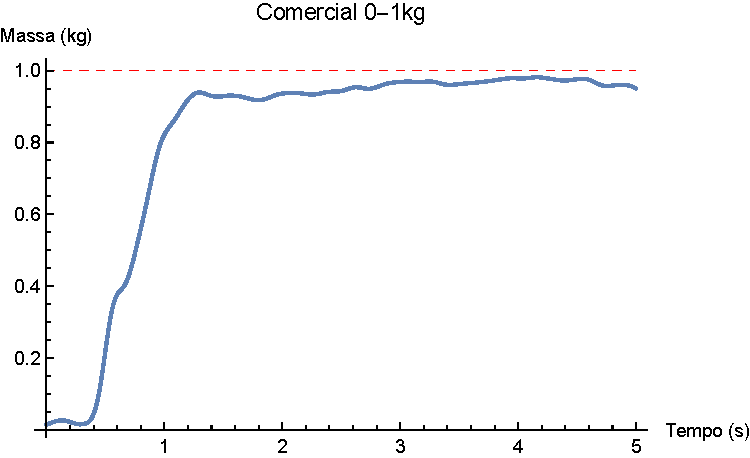
\includegraphics[width=\textwidth]{Comercial_0-1kg.pdf}
\caption{Curva temporal da resposta da célula de carga comercial quando adicionada uma carga de 1kg na célula em repouso.}
\label{fig:celula-comercial-resultado-0-1kg}
\end{figure}

Na Figura \ref{fig:celula-comercial-resultado-0-1kg} é possível observar que o tempo de resposta é baixo, de fato, nem é perceptível o tempo que ele leva para responder, uma vez que o fator mais notável no formato da curva não é a resposta do sensor nem da viga, mas a forma de como a carga era solta na viga. Era necessário segurar o peso para que a vibração do peso tivesse menor impacto na medida e este processo demorava aproximadamente 1 segundo como pode ser visto na curva.

A Figura \ref{fig:celula-comercial-resultado-0-4kg} apresenta a resposta da célula quando adicionado um peso suspenso de $4 kg$ na barra. A curva foi filtrada por um filtro passa-baixas digital com frequência de corte de 5Hz para reduzir o efeito do ruído gerado pelo circuito de condicionamento.

\begin{figure}[H]
\center
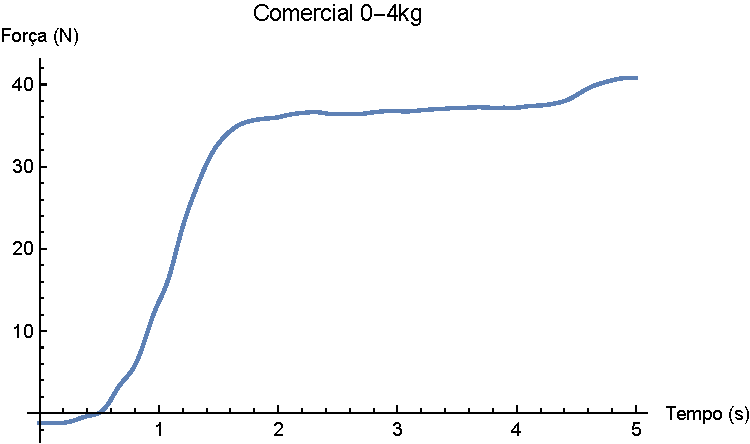
\includegraphics[width=\textwidth]{Comercial_0-4kg.pdf}
\caption{Curva temporal da resposta da célula de carga comercial quando adicionada uma carga de 4kg na célula em repouso.}
\label{fig:celula-comercial-resultado-0-4kg}
\end{figure}

A Figura \ref{fig:celula-comercial-resultado-0-4kg} é possível observar que a célula continua linear no intervalo de 4 kg e o valor de estabilidade da célula está muito próximo da 4kg ao final do tempo de 5 segundos. Entretanto, há um pequeno \textit{offset} no ponto de 0 kg que acredita-se ser devido à problemas no circuito de condicionamento. Esta hipótese não foi testada. A Figura \ref{fig:celula-comercial-resultado-0-4kg-etapa} apresenta um sistema equivalente ao da Figura \ref{fig:celula-comercial-resultado-0-4kg} contudo desta vez a massa foi adicionada em duas etapas, primeiramente somente 2kg foram suspensos e logo após mais uma segunda massa de 2kg foi suspensa, totalizando 4kg suspenso na viga. É possível ver claramente o tempo em que cada massa foi adicionada ao sistema.

\begin{figure}[H]
\center
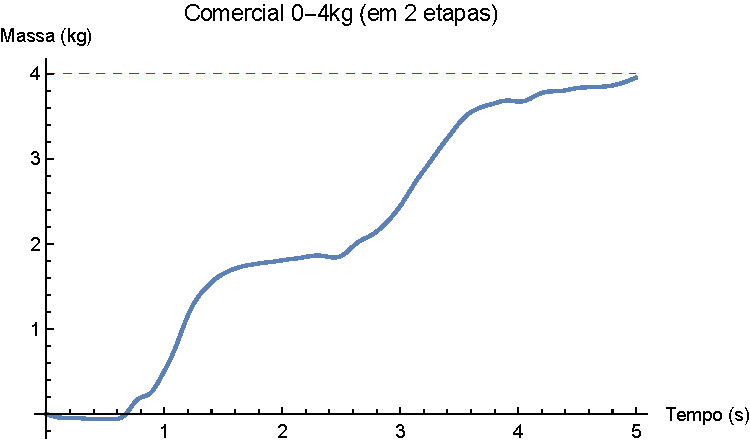
\includegraphics[width=\textwidth]{Comercial_0-4kg_etapa.pdf}
\caption{Curva temporal da resposta da célula de carga comercial quando adicionada uma carga de 4kg na célula em repouso em duas etapas (2kg + 2kg).}
\label{fig:celula-comercial-resultado-0-4kg-etapa}
\end{figure} 

A fim de validar a reprodutibilidade da célula, é necessário que a célula retorne ao ponto ponto de partida (0kg) quando as massas são removidas dos sistemas das Figuras \ref{fig:celula-comercial-resultado-0-4kg} e \ref{fig:celula-comercial-resultado-0-1kg}. A Figura \ref{fig:celula-comercial-resultado-1-0kg} apresenta a curva de resposta da célula quando uma carga de 1kg é removida.

\begin{figure}[H]
\center
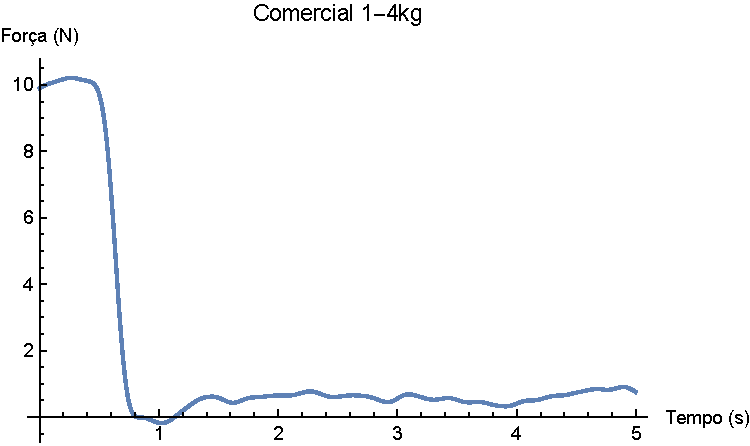
\includegraphics[width=\textwidth]{Comercial_1-0kg.pdf}
\caption{Curva temporal da resposta da célula de carga comercial quando se remove uma carga de 1kg.}
\label{fig:celula-comercial-resultado-1-0kg}
\end{figure}

Na Figura \ref{fig:celula-comercial-resultado-1-0kg} é possível observar que a resposta de remoção de carga é muito mais rápida do que a resposta de adição de carga, isto se dá ao fato de ser muito mais fácil (para o operador) remover a carga, pois basta que ele a eleve alguns centímetros ao invés de suspender onde ele deve ter cuidado para que não haja vibração que pode interferir com os resultados obtidos. Embora este efeito seja menos significante neste caso, ele ainda está presente em menor significância.

Outro fato interessante que é possível observar na Figura \ref{fig:celula-comercial-resultado-1-0kg} é o \textit{overshoot} presente ao redor da marca de 1 segundo. Acredita-se que este efeito é devido ao efeito elástico da viga, que ao ter a carga removida, se comporta como uma mola muito rígida e tem uma vibração muito rápida que logo se extingue devido à rigidez do material da célula de carga.

É possível dizer que a viga retornou ao valor inicial com a remoção da carga. É possível afirmar isto, pois a resolução de função de transferência medida foi de 0,2 kg e é possível observar que o valor final está ao redor do zero (isto é, está muito mais próximo do zero do que do 0,2kg).

A Figura \ref{fig:celula-comercial-resultado-4-0kg} apresenta a curva temporal de remoção de carga quando a viga está submetida à uma massa suspensa de 4kg e toda carga é removida de uma vez só.

\begin{figure}[H]
\center
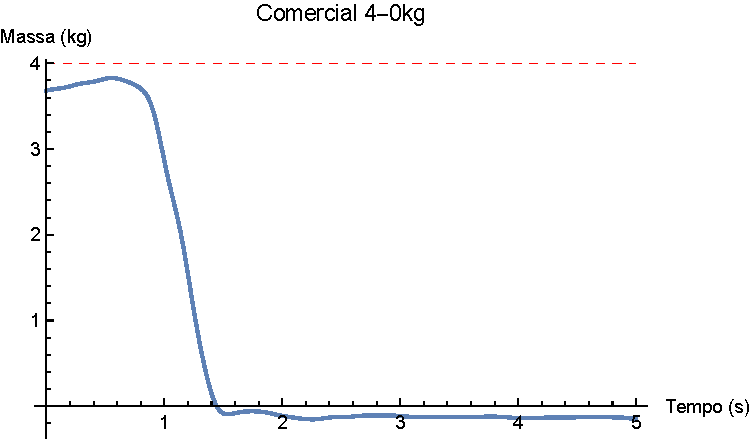
\includegraphics[width=\textwidth]{Comercial_4-0kg.pdf}
\caption{Curva temporal da resposta da célula de carga comercial quando se remove uma carga de 4kg.}
\label{fig:celula-comercial-resultado-4-0kg}
\end{figure}

Na Figura \ref{fig:celula-comercial-resultado-4-0kg} é menos visível o efeito elástico, embora este ainda esteja presente. Como na Figura \ref{fig:celula-comercial-resultado-1-0kg}, é possível afirmar que a célula retornou ao seu valor inicial e portanto o experimento teve sua reprodutibilidade confirmada.

\section{Célula de carga não-comercial}
A Tabela \ref{tab:celula-nao-comercial-resultado-funcao-transferencia} apresenta as medidas experimentais para a célula de carga não-comercial.


\begin{table}[H]
\centering
\caption{Tabela com os valores de medidos experimentalmente para ajuste da função de transferência experimental da célula de carga não-comercial.}
\begin{tabular}{|l|l|l|}

\hline
\textbf{Massa (kg)} & \textbf{Tensão Elétrica (V)} & \textbf{Tensão Elétrica (V)} \\ \hline
 0.0 & 1.273 & 1.272 \\ \hline
 0.2 & 1.262 & 1.261 \\ \hline
 0.4 & 1.249 & 1.253 \\ \hline
 0.6 & 1.242 & 1.244 \\ \hline
 0.8 & 1.233 & 1.233 \\ \hline
 1.0 & 1.226 & 1.225 \\ \hline
\end{tabular}
\label{tab:celula-nao-comercial-resultado-funcao-transferencia}
\end{table}

A função que melhor ajusta os dados da Tabela \ref{tab:celula-nao-comercial-resultado-funcao-transferencia} é dada na Equação \ref{eq:celula-nao-comercial-resultado-funcao-transferencia}

\begin{equation}
	m(V) = 27,0883 - 21,309 V
	\label{eq:celula-nao-comercial-resultado-funcao-transferencia}
\end{equation}

\noindent onde $m(V)$ é a massa em $kg$ a qual a célula de carga está submetida e $V$ é a tensão elétrica em $V$ medida na saída de ponte de Wheatstone com o sensor. A função foi ajustada com $R^2$ dado pela Equação \ref{eq:celula-nao-comercial-resultado-funcao-transferencia-r2}

\begin{equation}
	R^2 = 0.992582
	\label{eq:celula-nao-comercial-resultado-funcao-transferencia-r2}
\end{equation}

\todo{erro de linearidade}

A Figura \ref{fig:celula-nao-comercial-resultado-funcao-transferencia} apresenta um gráfico com a função de transferência da Equação \ref{eq:celula-nao-comercial-resultado-funcao-transferencia} e os dados da Tabela \ref{tab:celula-nao-comercial-resultado-funcao-transferencia}.

\begin{figure}[H]
\center
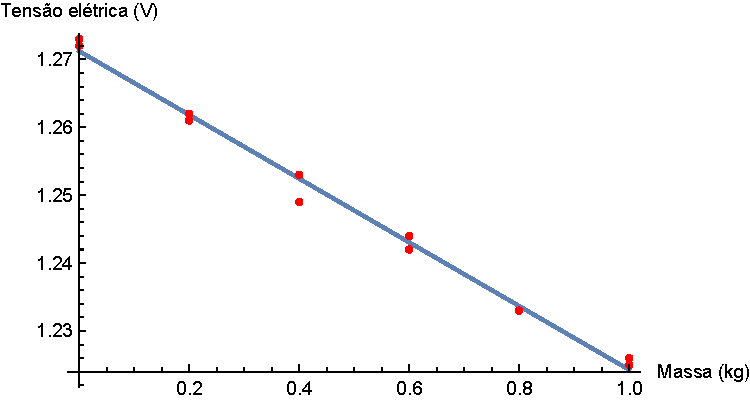
\includegraphics[width=\textwidth]{NaoComercial-Plot.pdf}
\caption{Função de transferência experimental: função de melhor ajuste e medidas experimentais}
\label{fig:celula-nao-comercial-resultado-funcao-transferencia}
\end{figure}

\noindent onde a linha contínua representa a função ajustada e os pontos representam cada medida individual realizada.

\subsection{Modelo computacional}


\subsection{Resposta temporal}

\begin{figure}[H]
\center
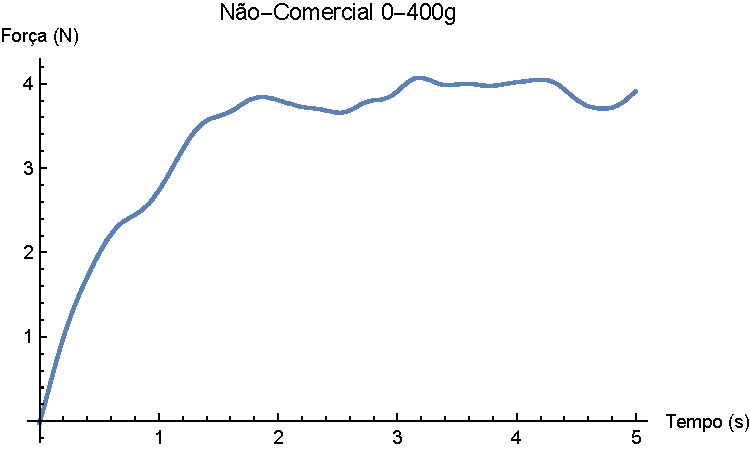
\includegraphics[width=\textwidth]{NaoComercial_0-400g.pdf}
\caption{Curva temporal da resposta da célula de carga não-comercial quando adicionada uma carga de 400g na célula em repouso.}
\label{fig:celula-nao-comercial-resultado-0-400g}
\end{figure}

\begin{figure}[H]
\center
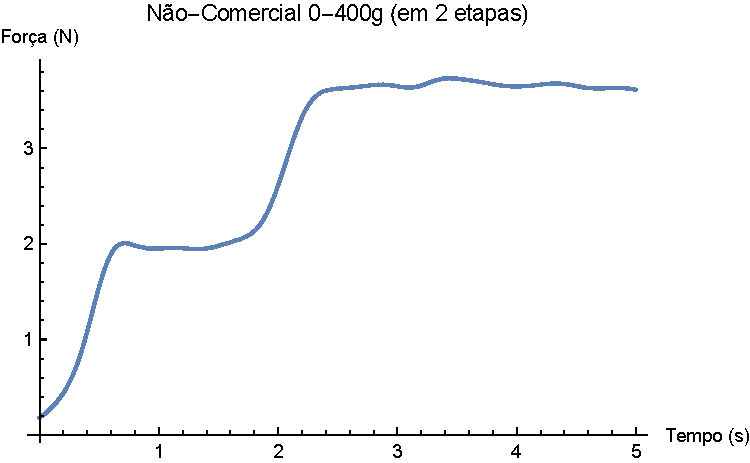
\includegraphics[width=\textwidth]{NaoComercial_0-400g_etapa.pdf}
\caption{Curva temporal da resposta da célula de carga não-comercial quando adicionada uma carga de 400g na célula em repouso em duas etapas (200g + 200g).}
\label{fig:celula-nao-comercial-resultado-0-400g-etapa}
\end{figure}

\begin{figure}[H]
\center
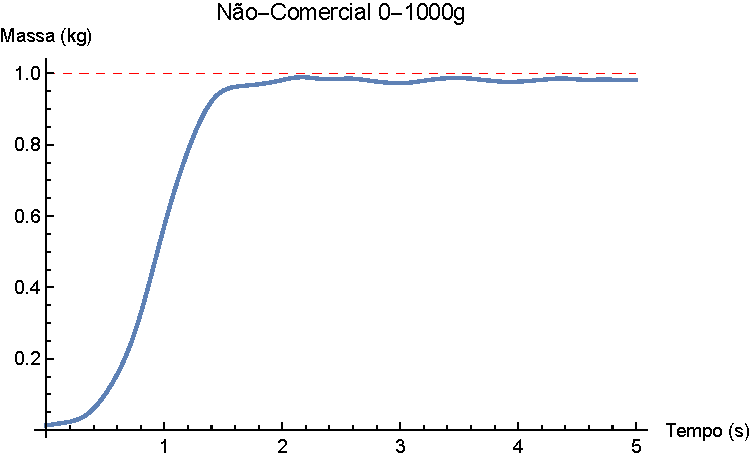
\includegraphics[width=\textwidth]{NaoComercial_0-1000g.pdf}
\caption{Curva temporal da resposta da célula de carga não-comercial quando adicionada uma carga de 1000g na célula em repouso.}
\label{fig:celula-nao-comercial-resultado-0-1000g}
\end{figure}

\begin{figure}[H]
\center
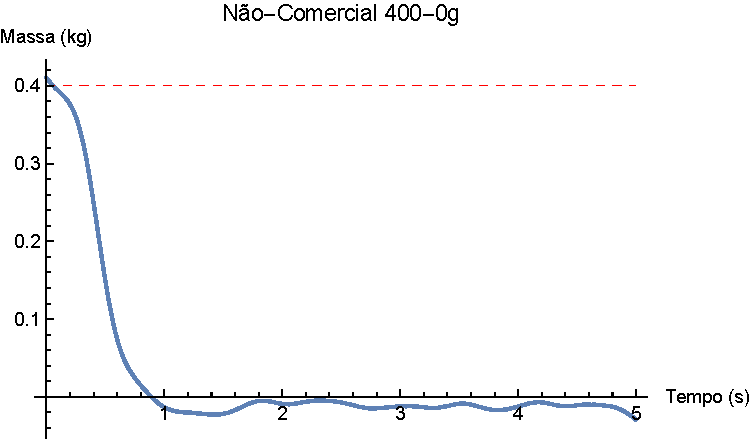
\includegraphics[width=\textwidth]{NaoComercial_400g-0.pdf}
\caption{Curva temporal da resposta da célula de carga comercial quando se remove uma carga de 400g.}
\label{fig:celula-nao-comercial-resultado-400-0g}
\end{figure}

\begin{figure}[H]
\center
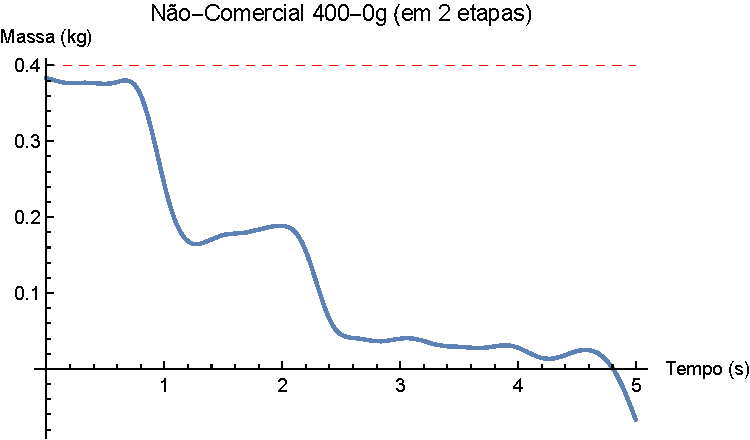
\includegraphics[width=\textwidth]{NaoComercial_400g-0_etapa.pdf}
\caption{Curva temporal da resposta da célula de carga comercial quando se remove uma carga de 400g em duas etapas (200g + 200g).}
\label{fig:celula-nao-comercial-resultado-400-0g-etapa}
\end{figure}

\begin{figure}[H]
\center
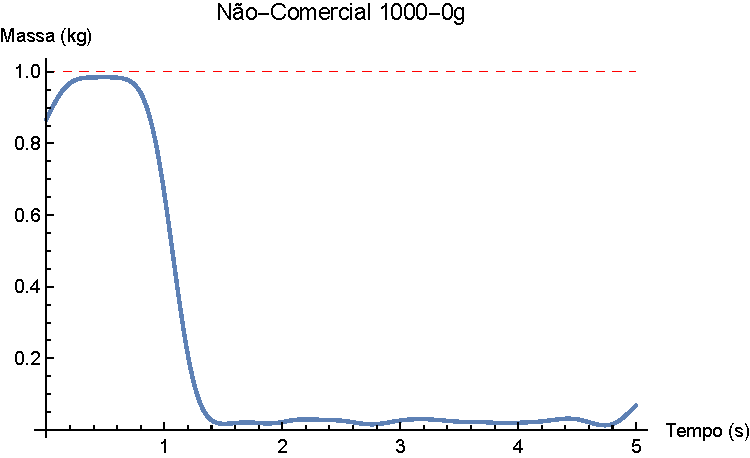
\includegraphics[width=\textwidth]{NaoComercial_1000g-0.pdf}
\caption{Curva temporal da resposta da célula de carga comercial quando se remove uma carga de 1000g.}
\label{fig:celula-nao-comercial-resultado-1000-0g}
\end{figure}

%%%%%%%%

\subsection{Efeito do aquecimento da viga}

\begin{figure}[H]
\center
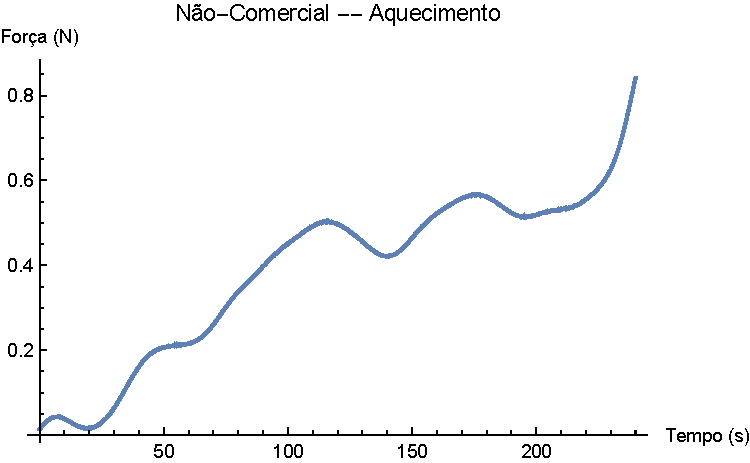
\includegraphics[width=\textwidth]{NaoComercial-Aquecimento.pdf}
\caption{Resposta temporal da célula de carga não-comercial para aquecimento de 4 minutos.}
\label{fig:celula-nao-comercial-resultado-aquecimento}
\end{figure}

\subsection{Análise de frequência fundamental}

\begin{figure}[H]
\center
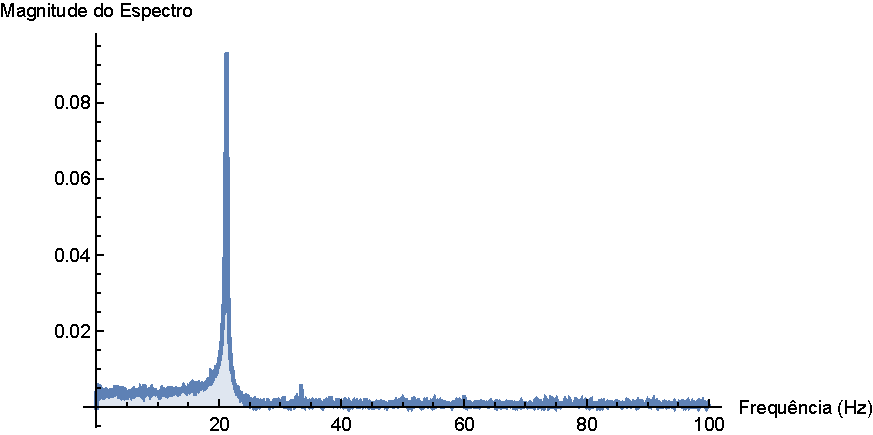
\includegraphics[width=\textwidth]{NaoComercial-Spectrum.pdf}
\caption{Espectro de frequência da célula de carga não-comercial quando submetida à uma batida. A curva de espectro foi suavizada por uma \textit{spline} de 3ª ordem.}
\label{fig:celula-nao-comercial-resultado-espectro}
\end{figure}

\begin{figure}[H]
\center
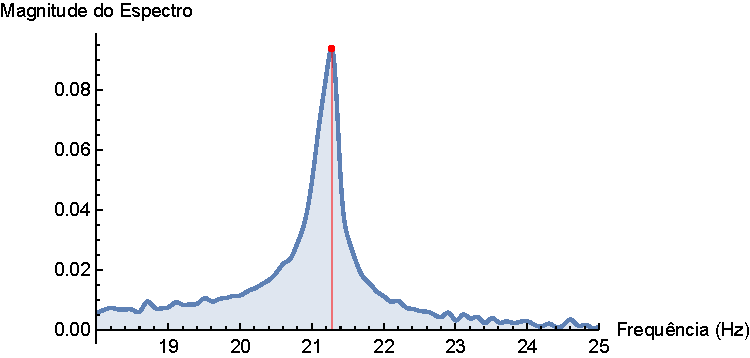
\includegraphics[width=\textwidth]{NaoComercial-SpectrumHighlight.pdf}
\caption{Destaque do espectro de frequência da célula de carga não-comercial (Figura \ref{fig:celula-nao-comercial-resultado-espectro}) quando submetida à uma batida e o pico máximo de frequência. A curva de espectro foi suavizada por uma \textit{spline} de 3ª ordem.}
\label{fig:celula-nao-comercial-resultado-espectro-destaque}
\end{figure}

\section{Torquímetro}

\chapter{Conclusões}


\todo{Tarefa no Laboratório: selecionar duas células disponibilizadas no laboratório de 
instrumentação (01 célula de carga não comercial do tipo viga engastada e 01 célula de carga comercial do tipo viga engastada – (para a célula de carga comercial ver Figuras 17 ou 18 e Tabelas 8 ou 9 – selecionar apenas 01 modelo da célula comercial)). Desenvolver usando o SolidWorks o correspondente modelo virtual e determinar o comportamento estático e dinâmico do modelo virtual para cada uma das células de carga. Observações: material da célula de carga não comercial é alumínio naval (várias células de carga, não comerciais, estão deformadas, mas mesmo assim trabalhar com as mesmas e suas não idealidades) e da célula comercial é Alumínio Anodizado. Limite de carga: 400g para a célula de carga não comercial e 5kg para a célula de carga comercial!}
\todo{Tarefa no Laboratório: selecionar a célula de carga (ver Figuras 19 e 20) disponibilizada no Laboratório de Instrumentação. Desenvolver usando o SolidWorks o correspondente modelo virtual e determinar o comportamento estático e dinâmico do modelo virtual. Observações: material da célula de carga é o aço inox AISI304 e a carga limite no eixo principal é de 250N. }
\todo{Tarefa no Laboratório: usando as duas células de carga (01 não comercial e outra comercial) do item i desenvolver um condicionador de sinais para cada célula de carga. Considerar a margem de carregamento mecânico utilizado na simulação (compatível com os limites de carga fornecidos no item i). Projetar e apresentar a Cadeia de Medida desenvolvida para cada célula de carga. Obter formas de onda no LabVIEW apresentando gráficos com escala e eixos adequados a aplicação. Sugestão: analisar a revisão bibliográfica deste laboratório para auxiliar o grupo no melhor projeto.}
\todo{Tarefa no Laboratório: considerando-se a célula de carga não comercial - do item anterior (com condicionador incluso): faça uma análise sobre o efeito da variação de temperatura nestas vigas. Como sugestão aplicar rapidamente uma fonte de calor na extremidade livre da célula de carga – LONGE DO EXTENSÔMETRO e verificar o comportamento de sua ponte. Sugestão: realize a aquisição destes dados.}
\todo{Drift (deriva): remover o maior peso padrão utilizado na calibração estática e imediatamente registrar Vo (registrar durante 5 minutos);}
\todo{Reprodução dos Valores: recolocar o maior peso padrão e registrar Vo. Remover o peso e imediatamente registrar Vo; }
\todo{Efeito do aquecimento: suavemente aquecer o topo da barra (sem carga). Registrar qualquer mudança em Vo enquanto aquece (não aquecer mais do que 10C e nunca sobre o strain-gage). Estimar a variação da temperatura. Aquecer a parte de baixo da barra e repetir os procedimentos anteriores deste item. Repetir novamente, porém aquecendo o topo e a parte de baixo da barra (ao mesmo tempo).}


\todo{Tarefa no Laboratório: considerando-se apenas a célula de carga não comercial (do item anterior): realizar o teste do impacto para determinar a frequência de ressonância dessa estrutura. Neste tipo de ensaio o padrão (e o correto) é utilizar um acelerômetro adequado, porém neste laboratório irão utilizar o(s) próprio(s) extensômetro(s). Utilizar uma placa de aquisição de dados (verificar se a entrada desta placa não será danificada pelo condicionador de vocês). Adquirir sinais no tempo durante a realização deste ensaio. Depois determinar a FFT deste sinal e discutir os resultados obtidos. Comparar com os dados da simulação dinâmica da célula de carga.}
\todo{Tarefa no Laboratório: considerando-se o torquímetro disponibilizado, no laboratório de instrumentação, projetar a cadeia de medição e o correspondente condicionamento. Apresentar seus resultados e comparar com os aspectos teóricos apresentados neste relatório.}

\todo{Faça uma comparação dos dados experimentais e/ou dos dados simulados e deste modelo. Discutir as suas diferenças.}

\todo{ladainha dos circuitos, de novo}

\newpage

\begin{thebibliography}{9}
\bibitem{mathematica-numerial-precision} \url{https://reference.wolfram.com/language/tutorial/NumericalPrecision.html}, acessado em 26 de abril de 2016
\bibitem{wikipedia-epsilon} \url{https://en.wikipedia.org/wiki/Machine_epsilon}, acessado em 26 de abril de 2016
\bibitem{livro-texto}  Balbinot, Alexandre; Brusamarello, Valner J., Instrumentação e Fundamentos de Medida - Vol.1 - 2ª Ed. Rio de Janeiro: LTC, 2014.
\bibitem{daq-specifications} NI USB-6009 -- DEVICE SPECIFICATIONS, \url{http://www.ni.com/pdf/manuals/375296a.pdf}, acessado em 3 de maio de 2016

\bibitem{daq-user-guide} NI USB-6009 -- USER GUIDE, \url{http://www.ni.com/pdf/manuals/371303n.pdf}, acessado em 3 de maio de 2016
\bibitem{datasheet-lm7805} Datasheet oferecido pelo fabricante do regulador de tensão elétrica LM7805CV, disponível em \url{http://www.datasheetlib.com/datasheet/221840/l7805cv_stmicroelectronics.html}.
\bibitem{datasheet-lm7905} Datasheet oferecido pelo fabricante do regulador de tensão elétrica LM7905, disponível em \url{http://www.ti.com/lit/ds/symlink/lm7905.pdf}.
\bibitem{datasheet-ref02} Datasheet oferecido pelo fabricante da referência de tensão elétrica REF02, disponível em \url{http://www.ti.com/lit/ds/sbvs003b/sbvs003b.pdf}.

\bibitem{datasheet-tl084} Datasheet oferecido pelo fabricante do amplificador operacional TL084, disponível em \url{http://www.ti.com.cn/cn/lit/ds/symlink/tl084.pdf}.

\bibitem{datasheet-ina126} Datasheet oferecido pelo fabricante amplificador de instrumentação INA126, disponível em \url{http://www.ti.com/lit/ds/symlink/ina126.pdf}.

\end{thebibliography}

\iftoggle{attachments}{
	\chapter*{Anexos}
	\label{ch:attachments}
	\section{Mathematica}
	
}

\end{document}
